\documentclass[10pt, conference, letterpaper]{IEEEtran}
\usepackage{cite}
\usepackage{xcolor,soul,framed}
\usepackage{amsmath,amssymb,amsfonts}
\usepackage{algorithmic}
\usepackage{graphicx}
\usepackage{color, soul}
\usepackage{svg}
\graphicspath{ {./images/} }

%---------------------------------------------------------------%
%-Include Graphics Macro:---------------------------------------%
% \begin{figure}[h]                                             %
%     \centering                                                %
%     \includegraphics[width=0.45\textwidth]{*}                 %
%     \caption{}                                                %
%     \label{fig:*}                                             %
% \end{figure}                                                  %
%-Include PDF Figures Macro:------------------------------------%
% \begin{figure}[h]                                             %
%     \centering                                                %
%     \includegraphics[width=0.45\textwidth, trim={0.5cm 0.5cm 0.5cm 0.5cm}, clip]{*.pdf}
%     \caption{}                                                %
%     \label{fig:*}                                             %
% \end{figure}                                                  %
%---------------------------------------------------------------%

\begin{document}

    %=============================== TITLE ===============================%
    \title{
        Meet-in-Future: Optimized Dispatching with Obsolete Information in Edge Computing System with MDP
    }
    \author{
        \IEEEauthorblockN{HONG Yuncong}
        \IEEEauthorblockA{
            \textit{Department of CS}, The University of Hong Kong, China \\
            ychong@cs.hku.hk
        }
    }
    \maketitle

    %============================== ABSTRACT ==============================%
    \begin{abstract}
        \label{sec:abstract}
        We formulate the problem with job dispatching in distributed Edge Computing system, and identify the difficulty exists in cooperation between APs (Access Points) and ESs (Edge Servers) with delayed information. In this work, we design the broadcast information in the system and formulate the corresponding problem into two-time-scale MDP problem.
    \end{abstract}

    \begin{IEEEkeywords}
        Edge Computing, Distributed Scheduling, Delayed Information, Collective Observability, Distributed Multi-agent MDP
    \end{IEEEkeywords}

    %============================ INTRODUCTION ============================%
    \begin{section}{INTRODUCTION}
        \label{sec:introduction}
        (in progress)

        Some traits to mention compared to related works:
        \begin{itemize}
            \item we don't accept communication cost in broadcast, because the global information to share requires both collective information and delayed information and the waiting time for scheduling should be avoided.
        \end{itemize}
    \end{section}

    %========================= LITERATURE REVIEW ==========================%
    \begin{section}{LITERATURE REVIEW}
        \label{sec:review}
        \begin{itemize}
            \item We use MDP definition in \cite{sutton1998introduction}
            \item The earliest related works we find is \cite{ref-01} (cited 167 times). In this work, the single agent is assumed not able to observe the global state, and thus they need communication to establish cooperation by sharing \emph{information}. The agent considers communication as extra action to synchronize the states and thus incurs extra cost. \\
            However, the communication is without delay, and converted into POMDP problem.
            \item The other work \cite{ref-02} considers continuous state observation with constant or stochastic delay with single agent. \\
            However, 
        \end{itemize}
    \end{section}

    %============================ FORMULATION =============================%
    \begin{section}{FORMULATION}
        \label{sec:formulation}

        In this section, we will firstly give out the definition of job dispatching models in the edge computing system. Then we illustrate the definition of the proposed optimization problem, and formulate it under MDP framework. The formulated distributed problem assumes APs apply their action independently on observation of broadcast information from other nodes with a reasonable broadcast design, and thus forms a collection of obsolete global states consensus on a global utility function. At last, we also give out the global problem definition with respect to our problem for comparison as upper bound.

        \begin{subsection}{Model Definition}
            In a Mobile Edge Computing (MEC) system, the mobile users would offload their computation jobs to the selected APs (Access Points) to the Edge Computing network. The APs would make decisions on each jobs to determine which ES (Edge Server) could better serve it and then dispatch jobs to the corresponding ES with a certain delayed time.
            
            In our problem, we consider the process of jobs from release until be fully processed. We identify the \emph{response time} of this process is mainly composed of: waiting time on AP to make decision, uploading time from AP to ES, and total computation-and-waiting time on ES.
            The details about the communication model and computation model for jobs will be elaborated in the following subsection. Moreover, to facilitate the cooperation among multiple APs, the well-designed broadcast is also elaborated in this section to help APs come to consensus on global states.
            
            \begin{subsubsection}{Communication Model}
                The communication model in our system ignores the underlaid physical property and MAC design. We focus on the communication process of uploading of jobs.
                The assumed uploading time is deterministic and known in advance when the job is released to AP. The uploading time for one job may variance with respect to different ESs from the arrived AP, and the distribution of variance is not known in advance but is guaranteed with an expectation.
                Moreover, we assume the uploading process could be parallel among jobs which implies infinite capacity, and the end-to-end time is domain by the propagation time and processing time rather than 
                \\
                As we are going to apply dispatching action for jobs on AP side, all the AP and ES nodes need to broadcast their jobs' information for cooperation. The broadcast delay is considered deterministic and asynchronous at their own pace.
                The details of broadcast design about interval and contents will be elaborated in the \textit{Global Optimization Problem} section.
                For now, we don't take the broadcast cost into consideration because it's not been easily evaluated in the complicated network model (without specified).
            \end{subsubsection}

            \begin{subsubsection}{Computation Model}
                We assume that there is only one job being computed at one time on the edge server. The computation model is assumed to be deterministic.
                Moreover, we assume unrelated parallel machine model which implies that the computation time for one job is known when released but has no relationship among the edge servers.
            \end{subsubsection}

            \begin{subsubsection}{Broadcast Model}

                \begin{itemize}
                    \item global aligned broadcast; interval is far larger than the maximum delay from one nodes to the other AP nodes;
                    \item consensus delay for $k$-th AP:
                        \begin{align}
                            \hat{d}_k = \max_{i\in(\mathcal{K}\cup\mathcal{N})}(d_{k,i})
                        \end{align}
                        and $\tau T + \hat{d}_k$ is the starting point of $\tau$-th stage for $k$-th AP;
                    \item Stage for $k$-th AP:
                        \begin{align}
                            (x_k={\tau})\triangleq t \in [\tau T^{br}+\hat{d}_k, (\tau+1) T^{br}+\hat{d}_k]
                        \end{align}
                        where $\tau$ is the general global state between $(\tau-1) T$-th and $\tau T$-th timeslot for all the AP nodes;
                    \item broadcast all of the information between the interval
                    \item 
                \end{itemize}

                The illustration figure \ref{fig:brd} for single broadcast includes several important time points which are also important in multiple asynchronous broadcast: $x_{k,*}, d_{k,*}, T^{br}_{k,*}$
                \begin{figure}[h]
                    \centering
                    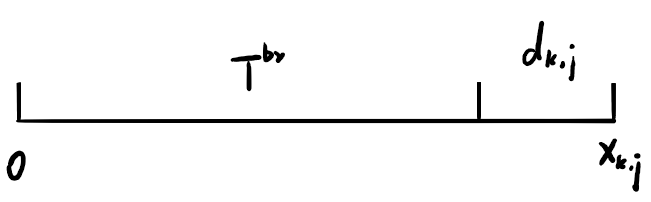
\includegraphics[width=0.45\textwidth]{single-broadcast.png}
                    \caption{Single broadcast timing illustration}
                    \label{fig:brd}
                \end{figure}
                And with the implication from the single broadcast, we generalize the conclusion for every broadcasts with:
                $$
                x_{k,*} = d_{k,*} + T^{Br}_{*}
                $$
                which takes a reasonable assumption that $T>d$ always ($*=k',n$ for $k$-th AP).

                Then we come up with the idea with collected broadcast states, which are split by the maximum broadcast interval which is denoted as $\hat{x}_k$:
                $$
                \hat{x}_k = \max(x_{k,*})
                $$
                And we denote all the partial or completed observed information (states of other nodes) in this smallest covering interval as $\Delta$.
                We notice that there is one periodic behavior as the broadcast interval is fixed for each node, and the period is simply obtained by LCM (Least Common Multiple):
                \begin{align*}
                    p_{k} &= \tilde{x}_k/\hat{x}_k
                    \\
                    \tilde{x}_k &= LCM(x_{k,*})
                \end{align*}
            \end{subsubsection}

        \end{subsection}

        \begin{subsection}{Problem Formulation}
            As we are considering broadcast delay, we could re-consider the broadcast information as partially observed collected information lasting for some time slots. We formulate the local MDP optimization problem with the same target as global value function, which means that each AP considers the global cost for cooperation but only takes action on itself. As the policy applied on each AP could not obtain the global information, we design the broadcast for every nodes to share their local information to other nodes (APs).
            
            Given that broadcast delay is fixed, the length vector of fractions would be also fixed.
            However, due to the broadcast delay, we could not optimize the original global optimization problem based on states on one single AP. So we develop the local MDP problem with collected broadcast information.

            \begin{figure}[h]
                \centering
                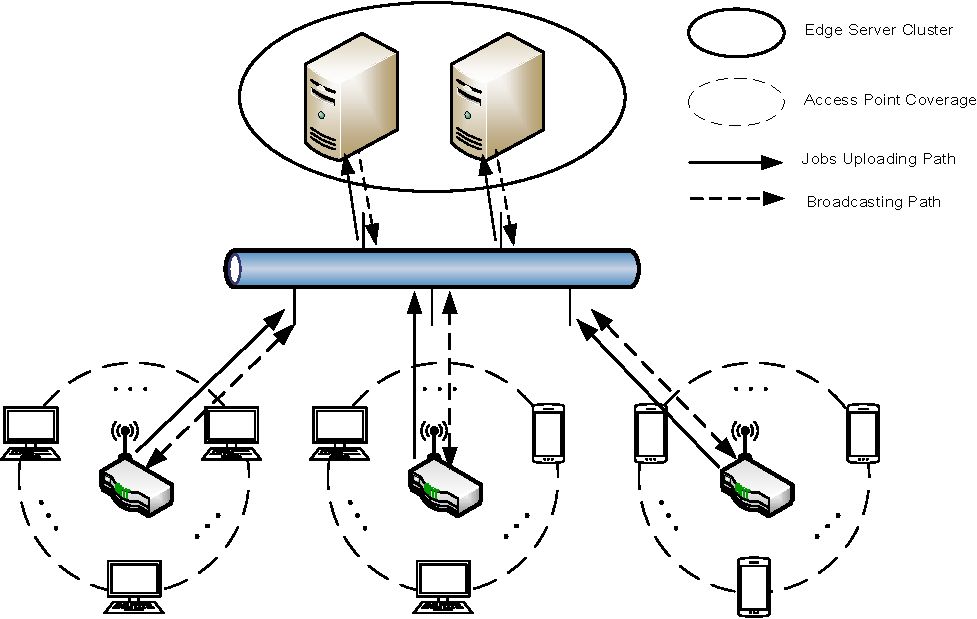
\includegraphics[width=0.45\textwidth, trim={0.5cm 0.5cm 0.5cm 0.5cm}, clip]{system-model.pdf}
                \caption{The Illustration of System Model}
                \label{fig:system}
            \end{figure}

            \begin{subsubsection}{Optimization Problem}
                We assume that there are $\mathcal{K}$ APs and $\mathcal{N}$ ESs in the MEC system.
                The arrival process of jobs at $k$-th AP is: $A^{(k)}(t)=I(t; (L_U, L_C))$ which is a indicator random process. It will return $0$ if no jobs arrive at $t$-th time slot, and return the job with property $(L_U, L_C)$ if one job arrives. $L_U, L_C$ are both vectors of length $\mathcal{N}$ denoting the deterministic uploading time and computation time respectively.
                $L_U$ is bounded by $T_U$ and $L_C$ is bounded by $T_C$, i.e. $L_U \in [1,T_U]$ and $L_C \in [1,T_C]$.
                \\
                For one job $j$, it will wait until the uploading decision is made for it; then it takes $L_U(n)$ time to be uploaded to $n$-th server; after uploaded, it will wait for its turn for computing until all the $L_C(n)$ components are processed and leave the system.
                \\
                Our optimization target is to minimize the average waiting time and computation time for each job, which is called the jobs' average response time. According to \emph{Little’s Law}, to minimize average response time, is equal to minimize the average number of jobs in a system, which is:
                \begin{gather}
                    \min_{\pi} \lim_{T \to \infty} E[\frac{1}{T} \sum_{t=0}^{T} N(t)]
                    \\
                    N(t) = \sum_{k \in \mathcal{K}} (A^{(k)}(t) + N_k(t))
                            + \sum_{n \in \mathcal{N}} N_n(t)
                \end{gather}
                where $N_k(t)$ denotes the number of jobs on $k$-th AP, and $N_n(t)$ denotes the number of jobs on $n$-th ES.
                The goal to minimize the cost caused by ESs could be simply achieved with heuristic algorithm \emph{SJF} (shortest-job first), because it is the fastest way to reduce number of jobs on the edge server. So, in the next MDP problems we will focus on the policy applied on AP side, and leave ES with fixed heuristic algorithm.
            \end{subsubsection}

            \begin{subsubsection}{Single-Step Transition}
                We adapt the description at grains of jobs and formulate the states into job sets at APs and ESs:
                \begin{gather*}
                    \mathbf{S}_g(t) \triangleq
                    \begin{Bmatrix}
                        S_{k}^{(W)}(t) = \{ (L_C) \}_{N_{k}^{(W)}}
                        \\
                        S_{k,n}^{(U)}(t)= \{ (L_C), L_{cd}^{(U)}(t) \}_{N_{k,n}^{(U)}}
                        \\
                        S_{n}^{(C)}(t)  = \{ L_{cd}^{(C)}(t) \}_{N_{n}^{(C)}}
                    \end{Bmatrix}
                    _{k \in [1,\mathcal{K}], n \in [1,\mathcal{N}]}
                \end{gather*}
                where $L_C$ is a constant vector of length $\mathcal{N}$ with each denoting the computation time of that job on each server; and $L^{(U)}_{cd}(t), L^{(C)}_{cd}(t)$ are countdowns for uploading and computing time remained for that job.
            
                \begin{figure}[h]
                    \centering
                    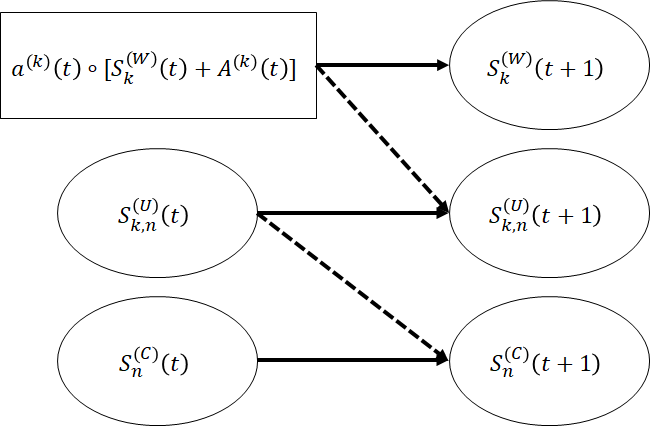
\includegraphics[width=0.45\textwidth]{single-transition.png}
                    \caption{Single-step transition function composing illustration}
                    \label{fig:trans}
                \end{figure}

                Firstly, we come up with some useful denotations for transmission expressed in figure \ref{fig:trans} as:
                \begin{align*}
                    I^{(W \to U)}_{k,n}(N;L) &\triangleq \{ (L_i),L^{(U)}_{cd}:=T^{br}_{k,n} \}_{i \in N}
                        \\
                    I^{(U \to C)}_{n}(N;L) &\triangleq \{ L^{(C)}_{cd}:=L_i \}_{i \in N}
                \end{align*}
                and we have the disturbance existing in the system as:
                \begin{gather*}
                    \Pr\{ I^{(W \to U)}(t) | S_{k}^{(W)}(t),A^{(k)}(t), a(t) \}
                    \\
                        = \Pr\{ A^{(k)}(t) \} \times \pi(a, S_g(t)|A^{(k)}(t))
                \end{gather*}
                where $I^{(W \to U)}(t)$ implies transition function for $S^{(W)}_{k}(t+1)$ and $S^{(U)}_{k,n}(t+1)$;

                The states transition on ES is easily obtained as following because the computation process on ES is deterministic:
                \begin{gather}
                    \Pr\{ S_{n}^{(C)}(t+1) |S_{n}^{(C)}(t), (S_{k}^{(U)}(t))_{k \in [1,\mathcal{K}]} \} = 1
                \end{gather}
                The other interesting properties exists in the situation that when only states of ES is presence and the constraints are inversely put on APs. With \emph{Bayes' Law}, we could have:
                \begin{align}
                    & \Pr\{ \sum{S_k(t)} | S_n(t,t+1) \} \nonumber\\
                    =& \frac{ \Pr\{\sum{S_k(t)}\} \cdot \Pr\{S_n(t,t+1)|\sum{S_k(t)}\} }{ \Pr\{S_n(t,t+1)\} } \nonumber\\
                    =& \frac{
                            \prod_k \Pr\{S_k(t)\}
                        }{
                            \Pr\{S_n(t,t+1)\}
                        }
                \end{align}
                where $S_n(t,t+1) \triangleq S_{n}^{(C)}(t+1) |S_{n}^{(C)}(t)$, and $\sum{S_k(t)} \triangleq \{S_{k}^{(U)}(t)\}_{k \in [1,K]}$.
            \end{subsubsection}

            \begin{subsubsection}{Multi-Step Transition}
                We adapt aligned broadcast in practice, and broadcast all the local information between the broadcast interval to establish consensus on the global states. And the agents would take action on the obsolete observed states.

                We denote the collective global states between broadcasts as:
                \begin{align}
                    & \Delta_1, \Delta_2, \Delta_3, \dots
                    \\
                    \text{where, } & \Delta_i \triangleq \{S(t)\}_{t \in [iT^{br},(i+1)T^{br})} \nonumber
                \end{align}
                and it stresses that each agent all maintains the same $\Delta_i$ for a $T^{br}$ period but not aligned, due to different consensus delay $\hat{d}_k$ on each agent.
                
                In this consensus formulation, we actually let every agents know the global states with different deterministic delay. The delayed information doesn't impact on global states formulation of MDP problem, but converted into delayed composed action. For example, the agent would take actions based both on global states $\Delta_1$ and $\Delta_2$ in the period of $\Delta_3$, because in the first half period it doesn't come to consensus on global states $\Delta_2$.

                We establish the following transition function for global states:
                \begin{align}
                    & \Pr\{\Delta_{i+1}, \Delta_{i} | \Delta_{i}, \Delta_{i-1}, \vec{\Omega}_k(\Delta_i), \vec{\Omega}_k(\Delta_{i-1})\}
                \end{align}
                where the output of policy $\Omega_k(\cdot)$ is a distribution of length $(\mathcal{N}+1)$ to determine the job uploading decision in the next $T^{br}$ period for $k$-th agent.

                This implies that: \hl{we cannot meet into future, but we can trace back into past}. The insight might be we have to maintain global consensus states to take action, and local states could no even come out with Markovian process.

                \begin{figure}[h]
                    \centering
                    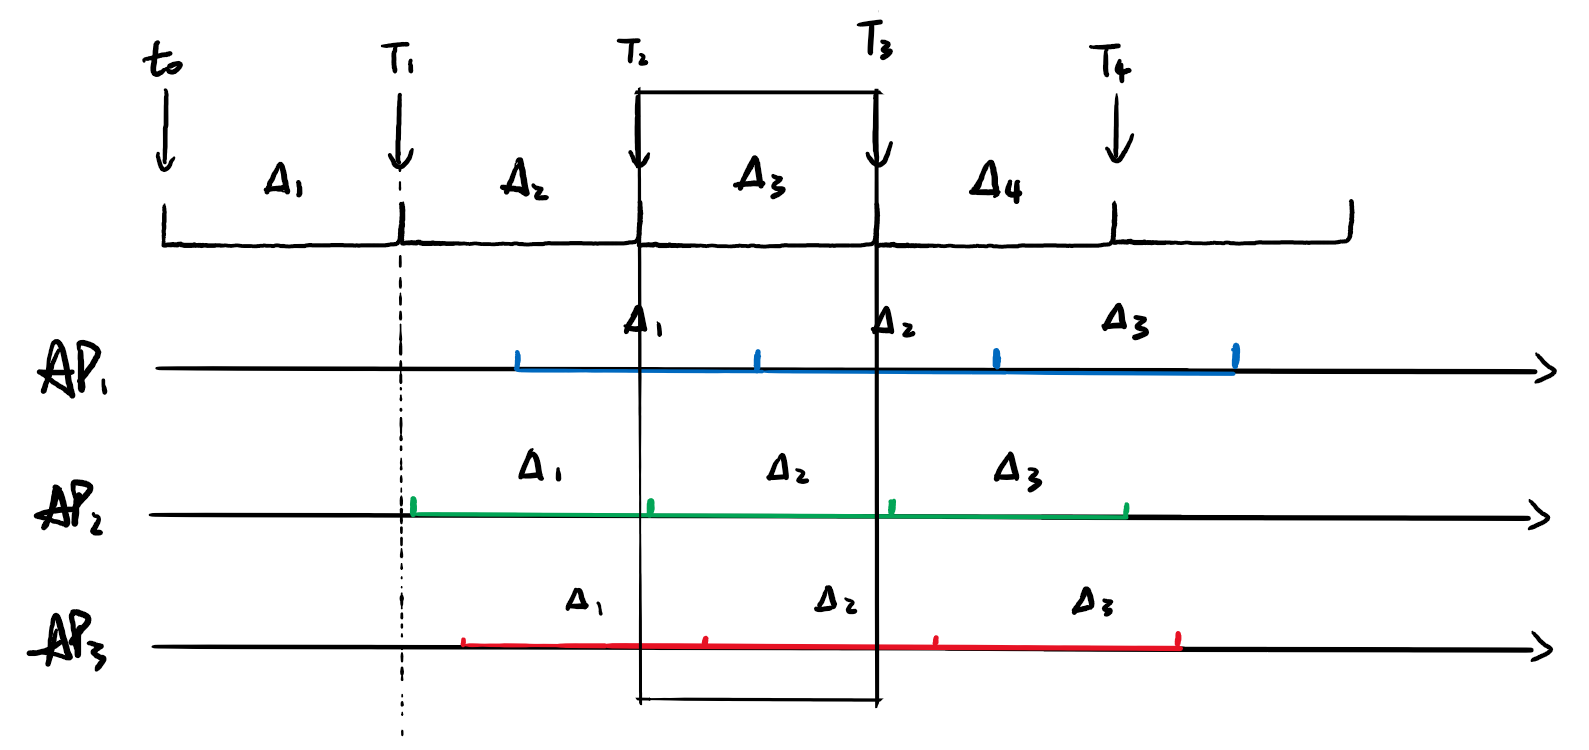
\includegraphics[width=0.45\textwidth]{broadcast-trans.png}
                    \caption{Global Consensus and Transition with Delayed Action}
                    \label{fig:br-trans}
                \end{figure}
                Then we have some notations for short expression of the transition from $\Delta_{i}$ to $\Delta{i+1}$ as:
                \begin{align}
                    P_k(T,a) &\triangleq \Pr\{ S^{(W,U)}_{k,D_T}|S^{(W,U)}_{k,D_1}, a_{\vec{D_T}},A^{(k)}_{\vec{D_T} }\}
                    \\
                    P_n(T) &\triangleq \Pr\{ S^{(C)}_{n,D_T}|S^{(C)}_{n,D_1}, S^{(U)}_{k,\vec{D_T}} \}
                \end{align}

                The transition function of states $\Delta_i$ is composed of multiple single-step transitions, and impacted by inner deduction constraints due to Bayes' Law. We firstly give out the rules for update, and explain why the mathematical expression for transition function would be complex and not readable.
                \\
                (The update rule algorithm:)
                \begin{enumerate}
                    \item Complement Step: \\
                    Firstly given ES constraints to extend AP states and complete other ES states not given, until the bound without ES constraints, $\max(\hat{d}_{k,n}^{(i-1)})$;\\
                    Then given fixed AP to deduct AP and completes ES states until bound of $R_i$, $\max(\hat{d}^{(i-1)}_{k,*})$;
                    \item Aligned Expansion Step: \\
                    Simply carry out multi-step transition lasting for $( \hat{x}^{(i)}_k - \max(\hat{d}^{(i)}_{k,*}) )$
                    \item Non-aligned Expansion Step: \\
                    Firstly extends AP states to the maximum bound $\hat{x}^{(i)}_k$; \\
                    Then complements needed ES states with \emph{Total Probability Theorem} and remove the un-needed AP states (the removal process is safe for the given states are removed after sum-up of total probability)
                \end{enumerate}
                Therefore, we could not easily write out the transition probability without the length of each broadcast information specified.
            \end{subsubsection}

        \end{subsection}

        \begin{subsection}{Global MDP Comparision}
            In this section, we give out the formulation of the global optimization problem with updated information under MDP framework. The algorithm for this problem would be trivial and 
            under the framework of MDP. In this section, we firstly ignore the obsolete information brought by the broadcast delay and assume a centralized agent could observe the global states in real-time. This formulation could help better understanding the structure of the problem and analyzing the optimality gap from the real localized optimization elaborated in next section.

            \begin{subsubsection}{Cost Function and Bellman Equation}
                According to the optimization target, we have the cost-to-go expression as followed:
                $$
                c(t) = \sum_{k \in \mathcal{K}}{|S^{(W)}_{k}(t)|}
                        + \sum_{k \in \mathcal{K}}\sum_{k \in \mathcal{N}}{|S^{(U)}_{k,n}(t)|}
                        + \sum_{k \in \mathcal{N}}{|S^{(C)}_{n}(t)|}
                $$
                The value equation in Bellman Equation format is as followed:
                $$
                V^{\pi}(S_g) = \sum_{S'_g} T(S_g, \pi(S_g), S'_g) (C(S_g') + \gamma V^{\pi}(S'_g))
                $$
                (need modification) where the dimension of possible $S'_g$ is:
                $$
                1 \times \sum{2^{|S^{(W)}_k|}} + (T_C \times T_U) \times \sum{2^{|S^{(W)}_k|+1}}
                $$
                and $C(S'_g)$ is the expectation of $c(t)$ given the arrival process as:
                \begin{align*}
                    C(S'_g) &= E[c(t)|(A^{(k)}(t))_{k \in [1,\mathcal{K}]}]
                    \\
                    &= 
                \end{align*}
            \end{subsubsection}
        \end{subsection}
        
    \end{section}

    %============================= ALGORITHM ==============================%
    \begin{section}{ALGORITHM}
        \label{sec:algorithm}
        (in progress)
    \end{section}

    %============================ EVALUATION ==============================%
    \begin{section}{EVALUATION}
        \label{sec:evaluation}
        (in progress)
    \end{section}

    %============================= CONCLUSION =============================%
    \begin{section}{CONCLUTION}
        \label{sec:conclusion}
        The future work to mention:
        \begin{itemize}
            \item broadcast failure
            \item randomized broadcast delay
        \end{itemize}
    \end{section}

    %============================== REFERENCE =============================%
    \bibliographystyle{IEEEtran}
    \bibliography{main.bib}
\end{document}